\documentclass[11pt,openany]{book}
\usepackage{blindtext}
\usepackage{tikz,tcolorbox}
\usepackage{xcolor}
\usepackage{amsfonts}
\usepackage{hyperref} 
\usepackage{indentfirst}
\usepackage{graphicx}
\usepackage[normalem]{ulem}
\usepackage [english]{babel}
\usepackage [autostyle, english = american]{csquotes}
\usepackage{appendix}
\usepackage{tabularx}
\usepackage{amsmath,amssymb}
\usepackage{mathtools}
\usepackage{makecell}
\graphicspath{ {./images/} }
\usepackage{enumitem}
\usepackage{soul}
\usepackage{mathtools}
\usepackage{wrapfig}
\usepackage{mathrsfs}
\usepackage{centernot}
\usepackage{amsthm}
\usepackage{listings}
\usepackage{biblatex}
\addbibresource{bibliograph.bib}

\usepackage{pagenote}


\definecolor{codegreen}{rgb}{0,0.6,0}
\definecolor{codegray}{rgb}{0.5,0.5,0.5}
\definecolor{codepurple}{rgb}{0.58,0,0.82}
\definecolor{backcolour}{rgb}{0.95,0.95,0.92}

\lstdefinestyle{mystyle}{
	backgroundcolor=\color{backcolour},   
	commentstyle=\color{codegreen},
	keywordstyle=\color{magenta},
	numberstyle=\tiny\color{codegray},
	stringstyle=\color{codepurple},
	basicstyle=\ttfamily\footnotesize,
	breakatwhitespace=false,         
	breaklines=true,                 
	captionpos=b,                    
	keepspaces=true,                 
	numbers=left,                    
	numbersep=5pt,                  
	showspaces=false,                
	showstringspaces=false,
	showtabs=false,                  
	tabsize=2
}

\lstset{style=mystyle}
%% End notes to be printed as sections at the
%% end of each chapter.
\renewcommand*{\notedivision}{\section*{\notesname}}
\renewcommand*{\pagenotesubhead}[1]{}

\newcommand*{\exercises}{\section*{\exercisename}}
%%%%%%%%%%%%% For customising the endnote markers. Comment these out if you don't want them.
% To prefix each note number with the chapter number
\renewcommand{\thepagenote}{\thechapter-\arabic{pagenote}}

% To have a slightly different formatting for the endnote numbers in the text -- smaller text, sans-serif, square brackets
\renewcommand\notenumintext[1]{\space{\footnotesize\sffamily[FN-#1]}}

% To have a slightly different formatting for the endnote numbers in the notes section. Just the square brackets and sans-serif; normal size.
\renewcommand\notenuminnotes[1]{{\sffamily[FN-#1] }}

% If you want a different name/heading for the end notes
\renewcommand{\notesname}{End Notes}
\newcommand{\exercisename}{Exercises}
%%%%%%%%%%%%% End customisation

\newcommand{\definition}[2]{\begin{tcolorbox}[title=Definition ({#1}),colframe=black]{#2}\end{tcolorbox}
}
\newcommand{\proposition}[1]{\begin{tcolorbox}[title=Proposition,colframe=red!50!blue!20!white,colback=red!35!blue!10!white, coltitle=black]{#1}\end{tcolorbox}
}
\newcommand{\theorem}[2]{\begin{tcolorbox}[title=Theorem ({#1}),colframe=red!70!black,colback=red!5!white]{#2}\end{tcolorbox}
}
\newcommand{\example}[1]{\begin{tcolorbox}[title=Example,colframe=yellow!50!white,colback=yellow!20!white,coltitle=black]{#1}\end{tcolorbox}
}
%\newcommand{\exercises}{\section*{\exercisename}}
%% THIS LINE IS MANDATORY
\makepagenote

\begin{document}
	
	\chapter{Sample - vector calculus}
	
	%in the actual thing, would ideally create a macro to have piecewise smooth reference the definition (in pdf
	
	In this chapter, we start with line integrals, and gradually build towards the analogous theorem of the fundamental theorem of calculus.
	
	\definition{Line Integral - scalar}{
		Let $U \subset \mathbb{R}^n$, $\gamma \subset U$ be a piecewise smooth curve, and $f: U \to \mathbb{R}$. The \textbf{line integral of $f$ along $\gamma$} is defined as
		\[
		\int_\gamma \ f \ ds \ = \ \int_a^b f(r(t)) \ |r'(t)| \ dt
		\]
		where $r : [a,b] \to \gamma$ is any parameterization of $\gamma$.
	}
	\definition{Line Integral - vector}{
		Let $U \subset \mathbb{R}^n$, $\gamma \subset U$ be a piecewise smooth curve, and $f: U \to \mathbb{R}^n$. The \textbf{line integral of $f$ along $\gamma$} is defined as
		\[
		\int_\gamma \ f  \cdot ds \ = \ \int_a^b f(r(t)) \cdot r'(t)  \ dt
		\]
		where $r : [a,b] \to \gamma$ is any parameterization of $\gamma$.
	}
	
	The line integral does not depend on the parameterization of $\gamma$. One exercise will guide you through the proof.
	\section*{Geometric intuition}
	%todo - plot in python
	For a visualization, let's plot a 2D function (so visualizing the graph in 3D) in Python. We want to integrate the function $f(x,y)=\sin(x+y)$ along the the curve $y=x^3$ for $-1<x<1$. That is, we can parametrize this curve as $(t,t^3)$ for $t\in[0,1]$.
	\begin{lstlisting}[language=Python]
import matplotlib.pyplot as plt
import numpy as np
#create figure
ax = plt.figure().add_subplot(projection='3d')

#plot sin(x+y)
X,Y=np.meshgrid(np.linspace(-1,1,40), np.linspace(-1,1,40))
Z=np.sin(X+Y)
surface=ax.plot_surface(X, Y, Z, alpha=0.5,
label='graph surface')
ax.set_xlabel('x')
ax.set_ylabel('y')
ax.set_zlabel('sin(x+y)')

#plot the curve and the cross section to integrate
curve=np.linspace(-1,1,100)
plot_curve=ax.plot(curve, curve**3, 0,
label='cross section to integrate',color='red')
curvevalues=np.sin(curve+curve**3)
curveonsurface=ax.bar3d(curve, curve**3,0,
dx=0.01, dy=0.01, dz=curvevalues, alpha=0.5,
color='red')

plt.legend()
plt.show()
	\end{lstlisting}

	\begin{wrapfigure}{r}{0.6\textwidth} 
		\centering
		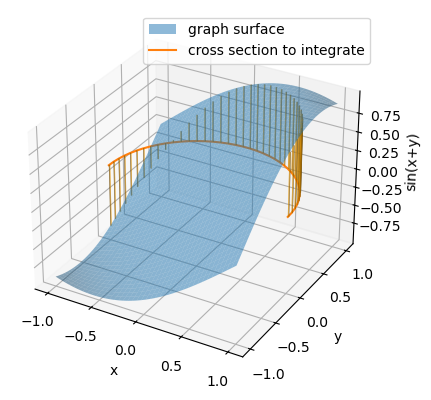
\includegraphics[width=0.6\textwidth]{sin.png}
	\end{wrapfigure}
	This scalar line integral represents the signed cross-section area of the graph along the curve, and is colored in orange on the left figure.
	What we need to do now is to unroll this cross section into 2D and perform a Riemann integral. However, a simple 
	\[
		\int_{-1}^{1} \ f(t,t^3) \ dt
	\]
	does not work - some parts of the curve are stretched and others are compressed. The red vertical bars are evenly spaced in t, but are denser near the origin. How much is this stretch/compression factor? It is represented by how quickly the curve is moving with respect to t, which is exactly $|r'(t)|$.
	
	For vector line integrals, we integrate the projection of $f$ onto the curve, so we can think of it as a scalar integral \[
		\int_a^b \left[ f(r(t)) \cdot \frac{r'(t)}{|r'(t)|}  \right]   |r'(t)| \ dt
	\]
	where the first term is the signed length of the projection of $f$ onto the tangent vector, and the second term is from the definition scalar line integrals.
	You might also recognize vector line integrals from the formula for work \[
	W = \int \vec{F} \cdot d\vec{s} 
	\]
	in first quarter physics. If we parametrize $\gamma$ as $\vec{r}(x)$ for $x \in [0,t]$, we get 
	\[
		W = \int_0^t \ \vec{F}(r(t)) \cdot \vec{r}'(t) dt
	\] 
	, work equals to the integral of power with respect to time!
	
	\exercises
	computation exercises follow...
	\begin{enumerate}
		\item The length of a curve can be obtained by integrating a constant with respect to ds. What is this constant that makes the cross section area equal (in value) to the arc length? 
		\item compute the length of the following curves : aaa, bbb, ccc
		\item compute the following line integrals : ddd, eee, fff
	\end{enumerate}
	
	\section*{Fundamental Theorem of Line Integrals}
	We want to build toward something that looks like 
	\[
		\int_{a}^{b} f(x) \ dx = F(b) - F(a)
	\], something similar in line integrals would be \[
		\int_\gamma f \cdot ds = F(b) - F(a)
	\] where $a$ and $b$ are the end points of $\gamma$. This is unfortunately not true from [one of the previous exercises]. So what can we do? We define this to be a property of a special set of vector-valued functions, and see what other properties this gives us.
	
	\definition{Conservative Vector Fields}{
		Let $U\subset\mathbb{R}^n$ be open+ other usual assumptions, and $f:U\to\mathbb{R}^n$. We say $f$ is \textbf{conservative} if there exists a function $F:U\to\mathbb{R}$ such that for every piecewise smooth curve $\gamma$ parametrized by $r: [a,b]\to U$
		\[
			\int_\gamma f \cdot ds = F(r(b)) - F(r(a)).
		\] 
	}
	Informally, $F$ is the antiderivative of $f$, and line integrals depend only $F$ evaluated on the endpoints of the curve.
	\proposition{
		If such an F exists, \[
			f = \nabla F.
		\]
	}
	\begin{proof} \ \\
		Idea: we consider the partial derivatives of $F$. Without loss of generality, it is enough to consider the partial derivative in the first variable $x$. \\
		Let $\vec{p} \in U$, we want to show that $\frac{\partial F}{\partial x} \big| _{\vec{p}} = f(\vec{p}) \cdot \vec{e}_1$. We can also consider the straight line $\gamma_h(t) = \vec{p} + t\vec{e}_1$ for $t\in[0,h]$. We then have \begin{align*}
			\frac{\partial F}{\partial x} \big| _{\vec{p}} &= \lim_{h\to 0} \frac{F(\vec{p}+h\vec{e}_1)-F(\vec{p})}{h} \\
			&= \lim_{h\to 0} \frac{\int_{\gamma_h} f \cdot ds}{h} \textrm{(definition of conservative vector field)}\\
			&= \lim_{h\to 0} \frac{\int_0^h f(\vec{p}+t\vec{e}_1) \cdot \vec{e}_1 \ dt}{h}
		\end{align*}
		The last expression is the (one dimensional) derivative of the function $g(t)=f(\vec{p}+t\vec{e}_1) \cdot \vec{e}_1$ at t=0, so equals $f(\vec{p})\cdot \vec{e}_1$ from the Fundamental Theorem of Calculus.
	\end{proof}
	
	As a bonus, we get the uniqueness of $F$.
	\proposition{
		If such an $F$ exists, it is unique up to addition of a constant.
	}
	\begin{proof}
		Let $G$ be another function that satisfies the equation in the definition of Conservative Vector Fields. Then $\nabla F - \nabla G = f-f =0$, so that $F-G$ is constant.
	\end{proof}
	
	\proposition{
	Let $f$ be conservative, and $\gamma_1$ and $\gamma_2$ be two curves with the same starting points and ending points. Then \[
		\int_{\gamma_1} f \cdot ds = \int_{\gamma_2} f \cdot ds
	\].
	For every closed curve $\gamma$,
	\[
	\int_\gamma f\cdot ds = 0
	\]
	}
	
	\begin{proof}
		By definition, note that closed curves have coinciding endpoints.
	\end{proof}
	These few properties are actually equivalent to the definition of conservative vector fields!
	\theorem{Fundamental Theorem of Line Integrals}{
		Let f... usual assumptions "Nice enough" $U$ connected open etc.\\
		The following are equivalent:
		\begin{enumerate}
			\item $f$ is conservative.
			\item $f = \nabla F$ for some $F:\mathbb{R}^n \to \mathbb{R}$.
			\item For every pair of curves $\gamma_1$ and $\gamma_2$ with the same starting points and ending points, \[
			\int_{\gamma_1} f \cdot ds = \int_{\gamma_2} f \cdot ds
			\]
			\item For every closed curve $\gamma$,
			\[
			\int_\gamma f\cdot ds = 0
			\]
		\end{enumerate}
	}
	\begin{proof}
		$1 \implies 2$, $1 \implies 3$, $1 \implies 4$ have been proved.\\
		$2 \implies 1$:\\
		Idea: we want to create an $F$ for an antiderivative, and there is already a candidate for $F$!
		Let's try to show that $F$ is indeed an antiderivative for $f$.
		Let $f=\nabla F$, and $gamma$ smooth parametrized by $r:[a,b]\to U$. Then
		\begin{align*}
			\int_\gamma f \cdot ds &= \int_\gamma \nabla F \cdot ds \\
			&= \int_a^b \nabla F(r(t)) \cdot r'(t) dt \\
			&= \int_a^b \frac{d \partial F(r(t))}{dt} \ dt \textrm{ (chain rule)}\\
			&= F(r(b)) - F(r(a)) \textrm{ (Fundamental Theorem of Calculus)}
		\end{align*} 
		The case where $\gamma$ is piecewise smooth is similar, you should get a telescoping series.
		$3 \implies 1$:\\
		We define $F$ by a line integral.
		Let $x \in U$, and $F(y) = \int_\gamma f \cdot ds$, where $\gamma$ is a (piecewise) smooth from $x$ to $y$.
		Because the integral is same regardless of the path, $F$ is well-defined.
		So that for every curve $\Gamma$that goes from $a$ to $b$, replace the line integral with a path $\gamma_1$ that goes from $a$ to $x$
		and $\gamma_2$ that goes from $x$ to $b$.
		so that \begin{align*}
			\int_\Gamma f\cdot ds &= \int_{\gamma_1} f\cdot ds + \int_{\gamma_2} f\cdot ds \\
			&= - (F(a) - F(x) ) + (F(x) + F(b))\\
			&= F(b) - F(a)
		\end{align*}
		$4 \implies 3$ is left as an exercise. 
	\end{proof}
	
	\example{
	Let $N$ be a positive integer, and set $\vec{p}_j = (j/N,j/N,j/N)$ for integers $0 \leq j < N$.
	Let $\gamma$ be the concatenation of lines $\vec{p}_j$ to $(\vec{p}_j+ 1/N \ \vec{e}_1)$,
	$(\vec{p}_j+ 1/N \ \vec{e}_1)$ to $(\vec{p}_j+ 1/N \ (\vec{e}_1 + \vec{e}_2))$, and 
	$(\vec{p}_j+ 1/N \ (\vec{e}_1 + \vec{e}_2))$ to $(\vec{p}_j+ 1/N \ (\vec{e}_1 + \vec{e}_2 + \vec{e}_3))$ for all $j$,
	Compute the line integral of $f(x,y,z)= (yz,xz,xy)$ along $\gamma$.
	}
	... what? $\gamma$ is intentionally complicated here, and you can definitely compute the integral as a summation of $3N$ line integrals.
	As a visualization exercise, try to predict what $\gamma$ looks like.
	\begin{lstlisting}[language=Python]
import matplotlib.pyplot as plt
import numpy as np
#create figure
fig=plt.figure(figsize=(5,4))
ax = fig.add_subplot(projection='3d')
N=10
p_j=[i/N for i in range(N)]
X=[j for i in p_j for j in [i,i+1/N,i+1/N] ]+[1]
Y=[j for i in p_j for j in [i,i,i+1/N] ]+[1]
Z=[j for i in p_j for j in [i,i,i] ]+[1]
plt.plot(X,Y,Z)
plt.show()
	\end{lstlisting}
	No one wants to do the annoying computation, so let's find another way.
	Could this be a conservative vector field? We need to find an antiderivative $F$ and evaluate it at the endpoints $(0,0,0)$ and $(1,1,1)$.
	We want something that is $yz$ differentiated with respect to (wrt) $x$, $xz$ differentiated wrt $y$, $xy$ differentiated wrt $z$.
	One solution is $F(x,y,z)=xyz$, which you can check very quickly it gives the correct partial derivatives.
	Now we apply the Fundamental Theorem of Line Integrals to show that
	\[
	\int_{\gamma} f\cdot ds = F(1,1,1) - F(0,0,0) = 1
	\]
	Elegant!
	\exercises
	\begin{enumerate}
		\item Complete the proof to the Fundamental Theorem of Line Integrals.
	\end{enumerate}
	
\end{document}